 \documentclass[a4paper,oneside,openany]{book}
\input{../Mod_base/base}
\input{../Mod_base/grafica}
\input{../Mod_base/rifIndici}
\input{../Mod_base/tcolorboxgest}
\input{../Mod_base/matematica}
\input{../Mod_base/tabelle}
\DeclareCaptionFormat{grafico}{\textbf{Grafico \thefigure}#2#3}
\DeclareCaptionFormat{esempio}{\textbf{Esempio \thefigure}#2#3}
\newcolumntype{L}{>{$\displaystyle}l<{$}}
\newcolumntype{C}{>{$\displaystyle}c<{$}}
\newcolumntype{R}{>{$\displaystyle}r<{$}}
\newcolumntype{T}{>{\centering\arraybackslash}p{1em}} 
\newcolumntype{W}{>{\sffamily\Large $}c<{$}}
%\newcolumntype{N}[1]{>{\centering\rule[-1mm]{0pt}{4.75mm}}m{#1}}
\newcolumntype{M}[1]{>{\centering}p{#1}}
\newcommand\pilH{\rule{0pt}{2.5ex}}
\newcommand\pilD{\rule[-1ex]{0pt}{0pt}}
\newlength{\gnat}
\newlength{\gnam}

\makeindex[options=-s ../Mod_base/oldclaudio.sti]
\input{../Mod_base/pagina}
\input{../Mod_base/indice}
\input{../Mod_base/date}
\input{../Mod_base/loghi}
\input{../Mod_base/unita_misura}
\input{../Mod_base/utili}
\input{../Mod_base/stand_class}


%per le semplificazioni
\usepackage{cancel}
\newcommand{\HRule}{\rule{\linewidth}{0.5mm}}

 \usepackage{placeins} 

\makeatletter
\renewcommand\frontmatter{%
	\cleardoublepage
	\@mainmatterfalse
	\pagenumbering{arabic}}
\renewcommand\mainmatter{%
	\cleardoublepage
	\@mainmattertrue}
\makeatother

\listfiles
%%%%%%%%%%%%%%%%%%%%%%%%%%%%%%%%
%%%lunghezza arrotondamenti%%%%%
\newcommand{\lungarrotandamento}{4}
%%%%%%%%%%%%%%%%%%%%%%%%%%%%%%%%%%

\usepackage{tkz-berge}
\begin{document}
\frontmatter
		\begin{titlepage}
	\begin{center}
		\input{../Mod_base/Lgrande}\\[1cm]
		\textsc{\LARGE Claudio Duchi}\\[1.5cm]
		\HRule \\[0.4cm]
		{ \huge \bfseries ESERCIZI SVOLTI DI MATEMATICA}\\[0.4cm]
	{\huge \bfseries 	QUINTO}
		\HRule \\[1.5cm]
		\vfill
	\end{center}
	\begin{center}
		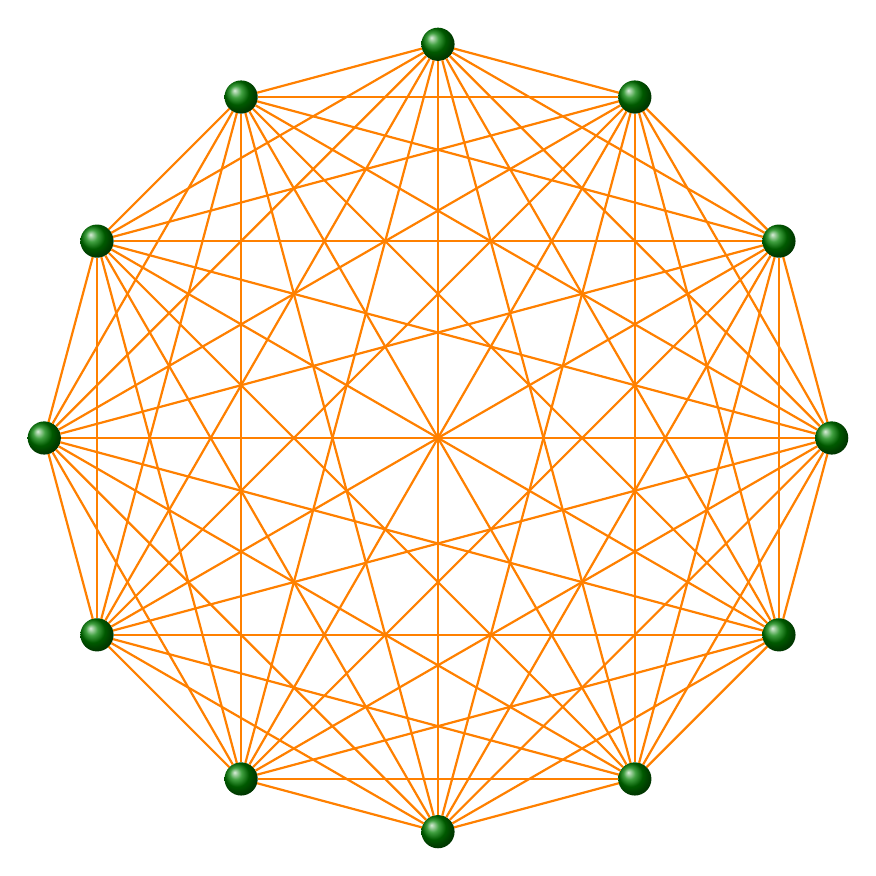
\begin{tikzpicture}
		\renewcommand*{\VertexBallColor}{green!50!black}
		\GraphInit[vstyle=Art]
		\grComplete[RA=5]{12}
		\end{tikzpicture}
	\end{center}
\end{titlepage}
\setcounter{page}{2}
\input{../Mod_base/copyright}
\tableofcontents 
%\addcontentsline{toc}{chapter}{\listtablename}
%\listoftables
\addcontentsline{toc}{chapter}{\listfigurename}
\listoffigures
\cleardoublepage\renewcommand\lstlistlistingname{Elenco esempi}
\addcontentsline{toc}{chapter}{\lstlistlistingname}
\addcontentsline{toc}{section}{Esempi}
\lstlistoflistings{}
\tcblistof[\section*]{thm}{Esempi}
\addcontentsline{toc}{section}{Contro esempi}
\tcblistof[\section*]{cthm}{Contro esempi}
\mainmatter%

\chapter{Limiti}
\section{Limite infinito per x che tende a valore finito}
\tcbstartrecording
%\begin{exercise}
%	\tcblower
%\end{exercise}
	%\begin{exercise}[no solution]
%	It holds:
%	\begin{equation*}
%	\frac{d}{dx}\left(\ln|x|\right) = \frac{1}{x}.
%	\end{equation*}
%\end{exercise}
\begin{exercise}
Calcoliamo il seguente limite
$\lim_{x\to 2^+}\dfrac{1}{x-2}$
	\tcblower
Calcoliamo il seguente limite
$\lim_{x\to 2^+}\dfrac{1}{x-2}$
	
Sostituendo due al denominatore otteniamo uno diviso zero. Possiamo risolvere l'esercizio in due modi. Primo metodo intuitivo, se sostituiamo all'incognita nel denominatore, valori leggermente superiori al due la differenza è positiva quindi \begin{equation*}
\lim_{x\to 2^+}\dfrac{1}{x-2}=+\infty
\end{equation*} Secondo metodo analitico. Studiamo, con una disequazione, il segno della frazione
\[x-2>0 \] 
otteniamo il grafico
\begin{center}
	\includestandalone{quinto/grafici/disprimogrado}
\end{center}\index{Limite!infinito!tende finito}
Quindi la frazione è positiva per valori a destra del due. Segue che 
\begin{equation*}
\lim_{x\to 2^+}\dfrac{1}{x-2}=+\infty
\end{equation*}
\end{exercise}
\begin{exercise}
Calcoliamo il limite 
	$\lim_{x\to -5^-}\dfrac{x-3}{x+5}$
	\tcblower
	Calcoliamo il limite 
	$\lim_{x\to -5^-}\dfrac{x-3}{x+5}$
	Sostituendo meno cinque al denominatore otteniamo meno otto diviso zero. Possiamo risolvere l'esercizio in due modi. Primo metodo intuitivo, sostituendo meno cinque all'incognita nel numeratore otteniamo un valore negativo. Procedendo in modo analogo al denominatore otteniamo un valore negativo (attenzione che consideriamo valori a sinistra di meno cinque). Quindi in numeratore e il denominatore sono entrambi negativi per cui la frazione a sinistra è positiva. Segue \begin{equation*}
	\lim_{x\to -5^-}\dfrac{x-3}{x+5}=+\infty
	\end{equation*} Secondo metodo analitico. Studiamo, con una disequazione, il segno della frazione
	\begin{align*}
	x-3>&0\\
	x>&3\\
	x+5>&0\\
	x>&-5
	\end{align*} 
	otteniamo il grafico
	\begin{center}
		\includestandalone{quinto/grafici/disprimogradodue}
	\end{center}\index{Limite!infinito!tende finito}
	Quindi la frazione è positiva per valori a sinistra di meno cinque. Segue che 
	\begin{equation*}
		\lim_{x\to -5^-}\dfrac{x-3}{x+5}=+\infty
	\end{equation*}
\end{exercise}
	\begin{exercise}[no solution]
Calcoliamo il limite
	$\lim_{x\to -3}\dfrac{2}{(x+3)^2}$

\end{exercise}
	\begin{exercise}[no solution]
Calcoliamo il limite
	$\lim_{x\to -2}\dfrac{2x}{(x+2)^2}$
\end{exercise}
	\begin{exercise}[no solution]
	Calcoliamo il limite
	$\lim_{x\to 0^-}\left(\dfrac{1}{x^3}+x\right)$
\end{exercise}
\section{Limite infinito per x che tende ad infinito}
\begin{exercise}
Calcoliamo il limite 
$\lim_{x\to +\infty}3x^3-x^2-x-1$
	\tcblower
	Calcoliamo il limite 
	$\lim_{x\to +\infty}3x^3-x^2-x-1$
Per valori di $x$ che tendono all'infinito le varie parti del polinomio tendono a più o meno infinito. Per ovviare a questa contraddizione procediamo come segue:
\begin{align*}
\lim_{x\to +\infty}3x^3-x^2-x-1=&\\
&=\lim_{x\to +\infty} x^3\left(3-\dfrac{x^2}{x^3}-\dfrac{x}{x^3}-\dfrac{1}{x^3}\right)\\
&=\lim_{x\to +\infty} x^3\left(3-\dfrac{1}{x}-\dfrac{1}{x^2}-\dfrac{1}{x^3}\right)
\intertext{i termini all'interno della parentesi tendono a tre mentre il termine all'esterno tende a più infinito quindi}
=&+\infty
\end{align*}\index{Limite!infinito!tende infinito}
\end{exercise}
	\begin{exercise}[no solution]
Calcoliamo il limite
$\lim_{x\to +\infty}3x^5+x^2-x+8$
\end{exercise}
\section{Forma indeterminata zero su zero}
\begin{exercise}
Calcoliamo il limite
$\lim_{x\to 1}\dfrac{x^2-1}{x-1}$
	\tcblower
Calcoliamo il limite
$\lim_{x\to 1}\dfrac{x^2-1}{x-1}$	
\begin{align*}
\lim_{x\to 1}\dfrac{x^2-1}{x-1}=\dfrac{0}{0}&
\intertext{scomponiamo il numeratore}
&=\lim_{x\to 1}\dfrac{(x-1)(x+1)}{x-1}
\intertext{semplificando}
&=\lim_{x\to 1}(x+1)\\
&=2
\end{align*}
\end{exercise}
\begin{exercise}
Calcoliamo il limite
$\lim_{x\to -2}\dfrac{2x^2+x-6}{4x^2+9x+2}$
	\tcblower
	Calcoliamo il limite
	$\lim_{x\to -2}\dfrac{2x^2+x-6}{4x^2+9x+2}$
	\begin{equation*}
\lim_{x\to -2}\dfrac{2x^2+x-6}{4x^2+9x+2}=\dfrac{0}{0}
\end{equation*}
Per risolvere questa forma indeterminata scomponiamo
il numeratore
\begin{align*}
2x^2+x-6=&0\\
x_{1,2}=&\dfrac{-1\pm\sqrt{1+48}}{4}\\
=&\dfrac{1\pm 7}{4}\\
=&\begin{cases}
x_1=-2\\
x_2=\dfrac{3}{2}
\end{cases}\\
2x^2+x-6=&2(x-\dfrac{3}{2})(x+2)
\intertext{scomponiamo
il denominatore}
4x^2+9x+2=&0\\
x_{1,2}=&\dfrac{-9\pm\sqrt{81-32}}{8}\\
=&\dfrac{-9\pm 7}{8}\\
=&\begin{cases}
x_1=-2\\
x_2=-\dfrac{1}{4}
\end{cases}\\
4x^2+9x+2=&4(x+\dfrac{1}{4})(x+2)
\intertext{quindi}
\lim_{x\to -2}\dfrac{2x^2+x-6}{4x^2+9x+2}=&\\
=&\lim_{x\to -2}\dfrac{2(x-\dfrac{3}{2})(x+2)}{4(x+\dfrac{1}{4})(x+2)}
\intertext{semplificando}
=&\lim_{x\to -2}\dfrac{2(x-\dfrac{3}{2})}{4(x+\dfrac{1}{4})}\\
=&\lim_{x\to -2}\dfrac{2x+3}{4x+1}\\
=&\dfrac{1}{7}
\end{align*}
\end{exercise}
\begin{exercise}
Calcoliamo il limite
$\lim_{x\to 1}\dfrac{2x^2+x-3}{x^2-x}$
	\tcblower
	Calcoliamo il limite
	$\lim_{x\to 1}\dfrac{2x^2+x-3}{x^2-x}$
\begin{equation*}
\lim_{x\to 1}\dfrac{2x^2+x-3}{x^2-x}=\dfrac{0}{0}
\end{equation*}
Per risolvere questa forma indeterminata scomponiamo
il numeratore
\begin{align*}
2x^2+x-3=&0\\ 
x_{1,2}=&\dfrac{-1\pm\sqrt{1+24}}{4}\\
=&\dfrac{1\pm 5}{4}\\
=&\begin{cases}
x_1=1\\
x_2=-\dfrac{3}{2}
\end{cases}\\
2x^2+x-3=&2(x+\dfrac{3}{2})(x-1)
\intertext{scomponiamo il denominatore}
x^2-x=&0\\
x_{1,2}=&\dfrac{1\pm\sqrt{1}}{2}\\
=&\dfrac{1\pm 1}{2}\\
=&\begin{cases}
x_1=0\\
x_2=1
\end{cases}\\
x^2-x=&x(x-1)
\intertext{quindi}
\lim_{x\to 1}\dfrac{2x^2+x-3}{x^2-x}=&\\
=&\lim_{x\to 1}\dfrac{2(x+\dfrac{3}{2})(x-1)}{x(x-1)}
\intertext{semplificando}
=&\lim_{x\to 1}\dfrac{2(x+\dfrac{3}{2})}{x}\\
=&\lim_{x\to 1}\dfrac{2x+3}{x}\\
=&5
\end{align*}
\end{exercise}
	\begin{exercise}[no solution]
	Calcoliamo il limite
	$\lim_{x\to 1}\dfrac{2x^2+5x-6}{x^2+x-2}$
\end{exercise}
\section{Forma indeterminata infinito su infinito}
\begin{exercise}
Calcoliamo il limite
$\lim_{x\to +\infty}\dfrac{2x-3}{1-5x}$
	\tcblower
	Calcoliamo il limite
	$\lim_{x\to +\infty}\dfrac{2x-3}{1-5x}$ Limite del tipo infinito su infinito, procediamo riscrivendo la frazione 
	\begin{align*}
\lim_{x\to +\infty}\dfrac{2x-3}{1-5x}=&\\
&=\lim_{x\to +\infty}\dfrac{x\left(2-\dfrac{3}{x}\right)}{x\left(\dfrac{1}{x}-5\right)}
\intertext{semplifico}
&=\lim_{x\to +\infty}\dfrac{2-\dfrac{3}{x}}{\dfrac{1}{x}-5}\\
&=-\dfrac{2}{5}
	\end{align*}
\end{exercise}
\begin{exercise}
Calcoliamo il limite
	$\lim_{x\to +\infty}\dfrac{x^2-3x+4}{x^2+x-6}$
	\tcblower
	Calcoliamo il limite
	$\lim_{x\to +\infty}\dfrac{x^2-3x+4}{x^2+x-6}$ Limite del tipo infinito su infinito, procediamo riscrivendo la frazione 
	\begin{align*}
	\lim_{x\to +\infty}\dfrac{x^2-3x+4}{x^2+x-6}=&\\
	&=\lim_{x\to +\infty}\dfrac{x^2\left(1-\dfrac{3x}{x^2}+\dfrac{4}{x^2}\right)}{x^2\left(1+\dfrac{x}{x^2}-\dfrac{6}{x^2}\right)}
	\intertext{semplifico}
	&=\lim_{x\to +\infty}\dfrac{1-\dfrac{3}{x}+\dfrac{4}{x^2}}{1+\dfrac{1}{x}-\dfrac{6}{x^2}}\\
	&=1
	\end{align*}
\end{exercise}
\begin{exercise}
Calcoliamo il limite 
$\lim_{x\to +\infty}\dfrac{x^2-x+1}{x^4-3x+4}$
\tcblower
Calcoliamo il limite 
$\lim_{x\to +\infty}\dfrac{x^2-x+1}{x^4-3x+4}$ Limite del tipo infinito su infinito, procediamo riscrivendo la frazione 
\begin{align*}
\lim_{x\to +\infty}\dfrac{x^2-x+1}{x^4-3x+4}=&\\
&=\lim_{x\to +\infty}\dfrac{x^2\left(1-\dfrac{x}{x^2}+\dfrac{1}{x^2}\right)}{x^4\left(1-\dfrac{3x}{x^4}+\dfrac{4}{x^4}\right)}
\intertext{semplifico}
&=\lim_{x\to +\infty}\dfrac{1-\dfrac{1}{x}+\dfrac{1}{x^2}}{x^2\left(1-\dfrac{3}{x^3}+\dfrac{4}{x^4}\right)}\\
&=0
\end{align*}
\end{exercise}
\begin{exercise}
Calcoliamo il limite 
	$\lim_{x\to +\infty}\dfrac{x^5-3x+1}{2x+1}$
	\tcblower
	Calcoliamo il limite 
	$\lim_{x\to +\infty}\dfrac{x^5-3x+1}{2x+1}$ Limite del tipo infinito su infinito, procediamo riscrivendo la frazione 
	\begin{align*}
	\lim_{x\to +\infty}\dfrac{x^5-3x+1}{2x+1}=&\\
	&=\lim_{x\to +\infty}\dfrac{x^5\left(1-\dfrac{3x}{x^5}+\dfrac{1}{x^5}\right)}{x\left(2+\dfrac{1}{x}\right)}
	\intertext{semplifico}
	&=\lim_{x\to +\infty}\dfrac{x^4\left(1-\dfrac{3}{x^4}+\dfrac{1}{x^5}\right)}{2+\dfrac{1}{x}}\\
	&=\infty
	\end{align*}
\end{exercise}
%\tcbstoprecording
%\newpage
%\section{Soluzione esercizi}
%\tcbinputrecords
%\newpage
\chapter{Asintoti}
\section{Asintoti verticali}
Risolvi i seguenti esercizi
\tcbstartrecording
%\begin{exercise}

%	\tcblower

%\end{exercise}
	%\begin{exercise}[no solution]
%	It holds:
%	\begin{equation*}
%	\frac{d}{dx}\left(\ln|x|\right) = \frac{1}{x}.
%	\end{equation*}
%\end{exercise}
\begin{exercise}[no solution]
	
	\begin{equation*}
	f(x)= \frac{2x^2+1}{x-1}.
	\end{equation*}
\end{exercise}
\begin{exercise}
\[y=\dfrac{x^2-5x+6}{x^2-1}\]
	\tcblower
Studio il dominio della funzione. 
\begin{align*}
x^2-1=&0\\ 
x_{1,2}=&\dfrac{0\pm\sqrt{0+4}}{2}\\
=&\dfrac{\pm 2}{2}\\
=&\begin{cases}
x_1=+1\\
x_2=-1
\end{cases}\\
\end{align*}
Quindi il dominio della funzione è  $x\neq\pm1$

Calcolo il limite
\begin{align*}
\lim_{x\to 1^+}\frac{x^2-5x+6}{x^2-1}=&\\
\intertext{Dato che}
(1^+)^2-1>&0\\
(1^+)^2-5\cdot 1^++6>&0\\
\intertext{otteniamo}
\lim_{x\to 1^+}\frac{x^2-5x+6}{x^2-1}=&+\infty\\
\end{align*} 
Calcolo il limite
\begin{align*}
\lim_{x\to 1^-}\frac{x^2-5x+6}{x^2-1}=&\\
\intertext{Dato che}
(1^-)^2-1<&0\\
(1^-)^2-5\cdot 1^++6>&0\\
\intertext{otteniamo}
\lim_{x\to 1^+}\frac{x^2-5x+6}{x^2-1}=&+\infty\\
\end{align*} 
quindi $x=1$ è un asintoto verticale.
Calcolo il limite
\begin{align*}
\lim_{x\to -1^+}\frac{x^2-5x+6}{x^2-1}=&\\
\intertext{Dato che}
(-1^+)^2-1<&0\\
(-1^+)^2-5\cdot (-1^+)+6>&0\\
\intertext{otteniamo}
\lim_{x\to 1^+}\frac{x^2-5x+6}{x^2-1}=&-\infty\\
\end{align*} 
Calcolo il limite
\begin{align*}
\lim_{x\to -1^-}\frac{x^2-5x+6}{x^2-1}=&\\
\intertext{Dato che}
(-1^-)^2-1>&0\\
(-1^-)^2-5\cdot (-1^-)+6>&0\\
\intertext{otteniamo}
\lim_{x\to 1^+}\frac{x^2-5x+6}{x^2-1}=&+\infty\\
\end{align*} 
quindi $x=-1$ è un asintoto verticale.
\end{exercise}
\begin{exercise}[no solution]
	
	\begin{equation*}
	f(x)= \frac{x^2+1}{x^2-4}.
	\end{equation*}
\end{exercise}
\begin{exercise}
	Trovare gli asintoti richiesti
\[y=\dfrac{3x^2+5x+2}{x^2-1}\]
	\tcblower
 il dominio
\begin{align*}
x^2-1=&0\\ 
x_{1,2}=&\dfrac{0\pm\sqrt{0+4}}{2}\\
=&\dfrac{\pm 2}{2}\\
=&\begin{cases}
x_1=+1\\
x_2=-1
\end{cases}\\
\end{align*}
Quindi il dominio della funzione è  $x\neq\pm1$

Calcolo il limite 
\begin{equation*}\lim_{x\to -1}\frac{3x^2+5x+2}{x^2-1}=\dfrac{0}{0}
\end{equation*}
Per risolvere questa forma indeterminata scompongo
il numeratore
\begin{align*}
3x^2+5x+2=&0\\
x_{1,2}=&\dfrac{-5\pm\sqrt{25-24}}{6}\\
=&\dfrac{-5\pm 1}{6}\\
=&\begin{cases}
x_1=-1\\
x_2=-\dfrac{2}{3}
\end{cases}\\
3x^2+5x+2=&3(x+\dfrac{2}{3})(x+1)
\end{align*}
quindi
\begin{align*}
\lim_{x\to -1}\dfrac{3x^2+5x+2}{x^2-1}=&\\
=&\lim_{x\to -1}\dfrac{3(x+\dfrac{2}{3})(x+1)}{(x-1)(x+1)}
\intertext{semplifico}
=&\lim_{x\to -1}\dfrac{3x+2}{x-1}\\
=&\dfrac{1}{2}
\end{align*}
Quindi $x=-1$ non è asintoto verticale. Utilizzando i calcoli precedenti otteniamo il limite:
\begin{equation*}
\lim_{x\to 1}\dfrac{3x^2+5x+2}{x^2-1}=\lim_{x\to 1}\dfrac{3x+2}{x-1}
\end{equation*}
Studio con una disequazione il segno della funzione
\begin{equation*}
y=\dfrac{3x+2}{x-1}\geq0
\end{equation*}
\begin{align*}
3x+2\geq&0\\
x\geq&-\dfrac{2}{3}\\
x-1>&0\\
x>&1
\end{align*}
otteniamo il grafico
\begin{center}
	\includestandalone{quinto/grafici/disprimogradodueb}
\end{center}\index{Limite!infinito!tende finito}
Quindi la frazione è positiva per valori a destra di uno negativa a sinistra. Segue che
\begin{align*}
\lim_{x\to 1^+}\dfrac{3x+2}{x-1}=&+\infty\\
\lim_{x\to 1^-}\dfrac{3x+2}{x-1}=&-\infty\\
\end{align*}
Quindi $x=1$ è asintoto verticale\index{Asintoto!verticale}
Potevamo procedere anche come segue:
 
Calcolo il limite
\begin{align*}
\lim_{x\to 1^+}\frac{3x+2}{x-1}=&\\
\intertext{Dato che}
1^+-1>&0\\
3\cdot (1^+)+2>&0\\
\intertext{otteniamo}
\lim_{x\to 1^+}\frac{3x+2}{x-1}=&+\infty\\
\end{align*} 
Calcolo il limite
\begin{align*}
\lim_{x\to 1^-}\frac{3x+2}{x-1}=&\\
\intertext{Dato che}
1^--1<&0\\
3\cdot (1^-)+2>&0\\
\intertext{otteniamo}
\lim_{x\to 1^-}\frac{3x+2}{x-1}=&-\infty\\
\end{align*} 
\end{exercise}
\begin{exercise}[no solution]
	
	\begin{equation*}
	f(x)= \frac{2x^2+x}{x^2+2x+1}.
	\end{equation*}
\end{exercise}
\begin{exercise}
	Trovare gli asintoti richiesti
\[y=\dfrac{x^2+4x+3}{x^2+3x+5}\]
	\tcblower
Determino il dominio ponendo il denominatore uguale a zero
\begin{align*}
x^2+3x+5=&0\\ 
x_{1,2}=&\dfrac{-3\pm\sqrt{9-20}}{2}\\
\intertext{L'equazione non ha soluzioni reali}
\end{align*}
La funzione non ha asintoti verticali
\end{exercise}
\begin{exercise}Trovare gli asintoti richiesti
\[y=\dfrac{3x^2+1}{x^3+x^2} \]
	\tcblower
\begin{align*}
x^3+x^2=&0\\ 
x^2(x+1)=0\\
x_{1,2}=&\dfrac{0\pm\sqrt{0+0}}{2}\\
=&0\\ 
x+1=&0\\
x_3=&-1
\end{align*}
Quindi il dominio è $x\neq 0$ e $x\neq-1$

Studio  il segno della funzione.
\[y=\dfrac{3x^2+1}{x^3+x^2} \]
Dato che è una razionale fratta studio il segno del numeratore 
\begin{align*}
3x^2+1=&0\\ 
x_{1,2}=&\dfrac{0\pm\sqrt{0-12}}{2}\\
\intertext{L'equazione non ha soluzioni reali}
\end{align*}
Utilizzando i risultati precedenti otteniamo il grafico 
\begin{center}
	\includestandalone{quinto/grafici/distreparti}
\end{center}
In base a quanto detto 
\begin{align*}
\lim_{x\to 0}\dfrac{3x^2+1}{x^3+x^2}=&+\infty\\
\lim_{x\to 1^-}\dfrac{3x^2+1}{x^3+x^2}=&-\infty\\
\lim_{x\to 1^+}\dfrac{3x^2+1}{x^3+x^2}=&+\infty\\
\end{align*}
Otteniamo lo stesso risultato nel seguente modo:
\begin{align*}
\lim_{x\to 0^+}\dfrac{3x^2+1}{x^3+x^2}=&
\intertext{Dato che}
3(0^+)^2+1>&0\\
x^3+x^2=&x^2(x+1)\\
(0^+)^2(0^++1)>&0
\intertext{otteniamo}
\lim_{x\to 0^+}\dfrac{3x^2+1}{x^3+x^2}=&+\infty
\end{align*}
continuiamo 
\begin{align*}
\lim_{x\to 0^-}\dfrac{3x^2+1}{x^3+x^2}=&
\intertext{Dato che}
3(0^-)^2+1>&0\\
x^3+x^2=&x^2(x+1)\\
(0^-)^2(0^-+1)>&0
\intertext{otteniamo}
\lim_{x\to 0^-}\dfrac{3x^2+1}{x^3+x^2}=&+\infty
\end{align*}
concludendo
\begin{align*}
\lim_{x\to -1^+}\dfrac{3x^2+1}{x^3+x^2}=&
\intertext{Dato che}
3(-1^+)^2+1>&0\\
x^3+x^2=&x^2(x+1)\\
(-1^+)^2(-1^++1)>&0
\intertext{otteniamo}
\lim_{x\to -1^+}\dfrac{3x^2+1}{x^3+x^2}=&+\infty
\end{align*}
continuiamo 
\begin{align*}
\lim_{x\to -1^-}\dfrac{3x^2+1}{x^3+x^2}=&
\intertext{Dato che}
3(-1^-)^++1>&0\\
x^3+x^2=&x^2(x+1)\\
(-1^-)^2(-1^-+1)<&0
\intertext{otteniamo}
\lim_{x\to -1^-}\dfrac{3x^2+1}{x^3+x^2}=&-\infty
\end{align*}
\end{exercise}
\begin{exercise}[no solution]
	
	\begin{equation*}
	f(x)= \frac{x+1}{2x-1}.
	\end{equation*}
\end{exercise}
\section{Asintoti orizzontali}
Risolvi i seguenti esercizi
\begin{exercise}
	Trovare gli asintoti richiesti
\[y=\dfrac{3x^2+5x+2}{x^2-1}\]
	\tcblower
Una funzione ha un asintoto orizzontale  se esiste ed è finito il limite
\begin{equation*}
\lim_{x\to +\infty}\dfrac{3x^2+5x+2}{x^2-1}
\end{equation*}
questo limite è del tipo $\dfrac{\infty}{\infty}$, forma indeterminata. 
\begin{align*}
\lim_{x\to +\infty}\dfrac{3x^2+5x+2}{x^2-1}=&\\
\lim_{x\to +\infty}\dfrac{x^2(3+5\dfrac{x}{x^2}+\dfrac{2}{x^2})}{x^2(1-\dfrac{1}{x^2})}=&
\intertext{semplifico}
\lim_{x\to +\infty}\dfrac{(3+5\dfrac{x}{x^2}+\dfrac{2}{x^2})}{(1-\dfrac{1}{x^2})}=&
\intertext{i termini fra parentesi sono trascurabili, quindi}
\lim_{x\to +\infty}\dfrac{(3+5\dfrac{x}{x^2}+\dfrac{2}{x^2})}{(1-\dfrac{1}{x^2})}=3\\
\end{align*}
l'asintoto è $y=3$\index{Asintoto!orizzontale}
\end{exercise}
	\begin{exercise}[no solution]
\[y=\dfrac{x^2+4x+3}{x^2+3x+5}\]
\end{exercise}
\begin{exercise}
	Trovare gli asintoti richiesti
	\[y=\dfrac{3x^2+1}{x^3+x^2} \]
	\tcblower
	\begin{align*}
	\lim_{x\to +\infty}\dfrac{3x^2+1}{x^3+x^2}=&\\
	\lim_{x\to +\infty}\dfrac{x^2(3+\dfrac{1}{x^2})}{x^3(1+\dfrac{1}{x})}=&
	\intertext{semplifico}
	\lim_{x\to +\infty}\dfrac{3+\dfrac{1}{x^2}}{x(1+\dfrac{1}{x})}=&
	\intertext{i termini fra parentesi sono trascurabili, quindi}
	\lim_{x\to +\infty}\dfrac{1(3+\dfrac{1}{x^2})}{x(1+\dfrac{1}{x})}=0\cdot 3=0\\
	\end{align*}
	L'asintoto è $y=0$, l'asse delle $x$.
\end{exercise}
\section{Asintoti obliqui }
Risolvere i seguenti esercizi
\begin{exercise}
	Trovare gli asintoti richiesti
	\[y=\dfrac{2x^3+x^2+2}{x^2+1}\]
	\tcblower
	\begin{align*}
	m=&\lim_{x\to +\infty}\dfrac{2x^3+x^2+2}{x^2+1}\cdot\dfrac{1}{x}\\
	=&\lim_{x\to +\infty}\dfrac{2x^3+x^2+2}{x^3+x}\\
	=&\lim_{x\to +\infty}\dfrac{x^3\left(2+\dfrac{1}{x}+\dfrac{2}{x^3}\right)}{x^3\left(1+\dfrac{1}{x^2}\right)}\\
	\intertext{Dato che}
	\dfrac{x^3}{x^3}=&1\\
	\lim_{x\to +\infty}\dfrac{1}{x}=&0\\
	\lim_{x\to +\infty}\dfrac{2}{x^3}=&0\\
	\lim_{x\to +\infty}\dfrac{1}{x^2}=&0\\
	\intertext{otteniamo}
	m=&2\\
	q=&\lim_{x\to +\infty}\left[\dfrac{2x^3+x^2+2}{x^2+1}-2x\right]\\
	=&\lim_{x\to +\infty}\dfrac{2x^3+x^2+2-2x^3-2x}{x^2+1}\\
	=&\lim_{x\to +\infty}\dfrac{x^2-2x+2}{x^2+1}\\
	=&\lim_{x\to +\infty}\dfrac{x^2\left(1-\dfrac{2}{x}+\dfrac{2}{x^2}\right)}{x^2\left(1+\dfrac{1}{x^2}\right)}\\
	\intertext{Dato che}
	\dfrac{x^2}{x^2}=&1\\
	\lim_{x\to +\infty}\dfrac{1}{x}=&0\\
	\lim_{x\to +\infty}\dfrac{1}{x^2}=&0\\
	\intertext{otteniamo}
	q=&1\\
	\intertext{Quindi l'asintoto è}
	y=&2x+1
	\end{align*}\index{Asintoto!obliquo}
\end{exercise}
\begin{exercise}[no solution]
	
	\begin{equation*}
	f(x)= \frac{2x^2+1}{x-1}.
	\end{equation*}
\end{exercise}
\begin{exercise}
	Trovare gli asintoti richiesti
	\[y=\dfrac{4x^4+1}{3x^3+1}\]
	\tcblower
	\begin{align*}
	m=&\lim_{x\to +\infty}\dfrac{4x^4+1}{3x^3+1}\cdot\dfrac{1}{x}\\
	=&\lim_{x\to +\infty}\dfrac{4x^4+1}{3x^4+x}\\
	=&\lim_{x\to +\infty}\dfrac{x^4\left(4+\dfrac{1}{x^4}\right)}{x^4\left(3+\dfrac{1}{x^3}\right)}\\
	\intertext{Dato che}
	\dfrac{x^4}{x^4}=&1\\
	\lim_{x\to +\infty}\dfrac{1}{x^3}=&0\\
	\lim_{x\to +\infty}\dfrac{1}{x^4}=&0\\
	\intertext{otteniamo}
	m=&\dfrac{4}{3}\\
	q=&\lim_{x\to +\infty}\left[\dfrac{4x^4+1}{3x^3+1}-\dfrac{4}{3}x\right]\\
	=&\lim_{x\to +\infty}\dfrac{12x^4+3-12x^4-4x}{3x^3+1}\\
	=&\lim_{x\to +\infty}\dfrac{-4x+3}{9x^3+3}\\
	=&\lim_{x\to +\infty}\dfrac{x\left(-4+\dfrac{3}{x}\right)}{x^3\left(9+\dfrac{3}{x^3}\right)}\\
	\intertext{Dato che}
	\dfrac{x}{x^3}=&\dfrac{1}{x^2}\\
	\lim_{x\to +\infty}\dfrac{3}{x}=&0\\
	\lim_{x\to +\infty}\dfrac{1}{x^2}=&0\\
	\lim_{x\to +\infty}\dfrac{3}{x^2}=&0\\
	\intertext{otteniamo}
	q=&0\\
	\intertext{Quindi l'asintoto è}
	y=&\dfrac{4}{3}x
	\end{align*}\index{Asintoto!obliquo}
\end{exercise}
\tcbstoprecording
\newpage
\section{Soluzioni asintoti}
\tcbinputrecords


%\opt{extra}{\input{extra}}
%\opt{grafici}{\input{grafici}}
\input{../Mod_base/MezziUsati}
\addcontentsline{toc}{chapter}{\indexname}
\printindex
\end{document}
